\documentclass[10pt]{article}

\usepackage[top=2cm, bottom=2cm, left=2cm, right=2cm]{geometry}
\usepackage{amsmath}
\usepackage{graphicx}
\usepackage{hyperref}
\usepackage[T1,LGR]{fontenc}
\usepackage[utf8]{inputenc}
\usepackage[greek,english]{babel}
\usepackage{alphabeta}
\usepackage{gensymb}
\usepackage{csquotes}
\usepackage[figurename=Εικόνα]{caption}
\renewcommand{\listfigurename}{Ευρετήριο εικόνων}
\usepackage{float}

\usepackage[bibencoding=auto,backend=biber,babel=other, style=numeric]{biblatex}
\addbibresource{references.bib}

\usepackage{listings}
\usepackage{minted}
\usemintedstyle{perldoc}
\usepackage{xcolor}
\urlstyle{same}

\title{Εκτίμηση μη-γραμμικού συστήματος με φίλτρο Kalman - Ανεστραμμένο εκκρεμές σε αμαξίδιο}
\author{Καραδήμος Αλέξιος}
\date{2020}


\begin{document}
%\begin{otherlanguage}{english}
\selectlanguage{greek}
\selectlanguage{english}

\begin{titlepage}

\newcommand{\HRule}{\rule{\linewidth}{0.5mm}} % Defines a new command for the horizontal lines, change thickness here

\center % Center everything on the page
 
%----------------------------------------------------------------------------------------
%	HEADING SECTIONS
%----------------------------------------------------------------------------------------

\textsc{\LARGE ΠΑΝΕΠΙΣΤΗΜΙΟ ΠΑΤΡΩΝ}\\[1.5cm] % Name of your university/college
\textsc{\Large Θεωρία εκτίμησης \& Στοχαστικός έλεγχος}\\[0.5cm] % Major heading such as course name
\textsc{\large \textlatin{ECE}ΔΚ803}\\[0.5cm] % Minor heading such as course title

%----------------------------------------------------------------------------------------
%	TITLE SECTION
%----------------------------------------------------------------------------------------

\HRule \\[0.4cm]
{ \huge \bfseries Εκτίμηση μη-γραμμικού συστήματος με φίλτρο Kalman - Ανεστραμμένο εκκρεμές σε αμαξίδιο}\\[0.4cm] % Title of your document
\HRule \\[1.5cm]
 
%----------------------------------------------------------------------------------------
%	AUTHOR SECTION
%----------------------------------------------------------------------------------------


% If you don't want a supervisor, uncomment the two lines below and remove the section above
%\Large \emph{Author:}\\
\emph{Αλέξιος Καραδήμος}\\ % Your name
Τμήμα Ηλεκτρολόγων Μηχανικών \& Τεχνολογίας Υπολογιστών\\[2cm]

%----------------------------------------------------------------------------------------
%	DATE SECTION
%----------------------------------------------------------------------------------------

{\large 2020}\\[1cm] % Date, change the \today to a set date if you want to be precise

%----------------------------------------------------------------------------------------
%	LOGO SECTION
%----------------------------------------------------------------------------------------

\begin{center}

\includegraphics[width=5cm]{images/up_2017_logo_gr.png}\\[1cm] % Include a department/university logo - this will require the graphicx package
\end{center}
 
%----------------------------------------------------------------------------------------

\vfill % Fill the rest of the page with whitespace

\end{titlepage}


%----------------------------------------------------------------------------------------
%	ΠΕΡΙΕΧΟΜΕΝΑ
%----------------------------------------------------------------------------------------

\renewcommand*\contentsname{Περιεχόμενα}
\tableofcontents


%----------------------------------------------------------------------------------------
%	ΠΕΡΙΓΡΑΦΗ ΣΥΣΤΗΜΑΤΟΣ
%----------------------------------------------------------------------------------------
\newpage

\section{Περιγραφή Συστήματος}

Το σύστημα που μελετάται σε αυτήν την εργασία είναι αυτό του ανεστραμμένου εκκρεμούς πάνω σε αμαξίδιο. Το σύστημα αυτό είναι ένα 
απλοποιημένο μοντέλο των αυτο-ισορροπημένων ρομποτ τύπου Segway (self-balancing robots).

\begin{center}
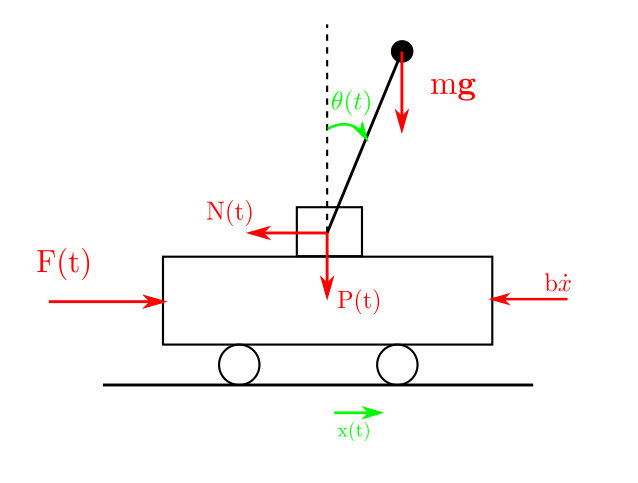
\includegraphics[width=10cm]{images/system.png}
\end{center}

Για τις δυνάμεις που ασκούνται στο αμαξίδιο έχουμε:
\[ Μ\ddot{x}(t) = F(t) - b\dot{x}(t) - N(t) \]
\[ N(t) = m\ddot{x} + ml\ddot{θ}(t)cosθ(t) - ml[\dot{θ}(t)]^2sinθ(t) \]
οπότε τελικά έχουμε
\[ (Μ+m)\ddot{x}(t) = F(t) - b\dot{x}(t) - ml\ddot{θ}(t)cosθ(t) + ml[\dot{θ}(t)]^2sinθ(t) \]

Για τις δυνάμεις που ασκούνται στο ανάστροφο εκκρεμές έχουμε:
\[ P(t)sinθ(t) + N(t)cosθ(t) - mgsinθ(t) = ml\ddot{θ}(t) + m\ddot{x}(t)cosθ(t) \]
\[ -P(t)sinθ(t) - N(t)cosθ(t) = I\ddot{θ}(t) \]
οπότε τελικά έχουμε
\[ (I+ml^2)\ddot{θ}(t) + mglsinθ(t) = - ml\ddot{x}(t)cosθ(t) \]



%----------------------------------------------------------------------------------------
%	ΓΡΑΜΜΙΚΟ ΜΟΝΤΕΛΟ ΧΩΡΙΣ ΘΟΡΥΒΟ
%----------------------------------------------------------------------------------------

\section{Γραμμικό μοντέλο χωρίς θόρυβο}

Αν υποθέσουμε οτι $$ θ(t) = π + φ(t) $$ όπου $$φ(t)$$ μικρή γωνία τότε $$ cosθ(t)=-1, sinθ(t) = -φ(t) $$ και $$ [\dot{θ}(t)]^2=0 $$
οπότε προκύπτει το γραμμικό μοντέλο

% TODO
\[
\begin{cases}
(Μ+m)\ddot{x}(t) = F(t) - b\dot{x}(t) + ml\ddot{φ}(t) \\
(I+ml^2)\ddot{φ}(t) - mglφ(t) = ml\ddot{x}(t)
\end{cases}
\]

\[
\begin{cases}
\dot{\vec{x}} = \mathbf{A}\vec{x} + \mathbf{B}u \\
\vec{y} = \mathbf{C}\vec{x} + \mathbf{D}u
\end{cases}
\]
όπου

\[
\vec{x} = 
\begin{bmatrix}
x \\ \dot{x} \\ θ \\ \dot{θ}
\end{bmatrix}
\] και

\[
\mathbf{A} =
\begin{bmatrix}
0 & 1 & 0 & 0 \\
0 & \frac{-(I+ml^2)b}{I(M+m)+Mml^2} & \frac{m^2gl^2}{I(M+m)+Mml^2} & 0 \\
0 & 0 & 0 & 1 \\
0 & \frac{-mlb}{I(M+m)+Mml^2} & \frac{mgl(M+m)}{I(M+m)+Mml^2} & 0 \\
\end{bmatrix}
\]

\[
\mathbf{B} =
\begin{bmatrix}
0 \\
\frac{-(I+ml^2)b}{I(M+m)+Mml^2} \\
0 \\
\frac{-(I+ml^2)b}{I(M+m)+Mml^2} \\
\end{bmatrix} \;\;
\mathbf{C} =
\begin{bmatrix}
1 & 0 & 0 & 0 \\
0 & 0 & 1 & 0 \\
\end{bmatrix} \;\;
\mathbf{D} =
\begin{bmatrix}
0 \\
0 \\
\end{bmatrix}
\]

\begin{center}
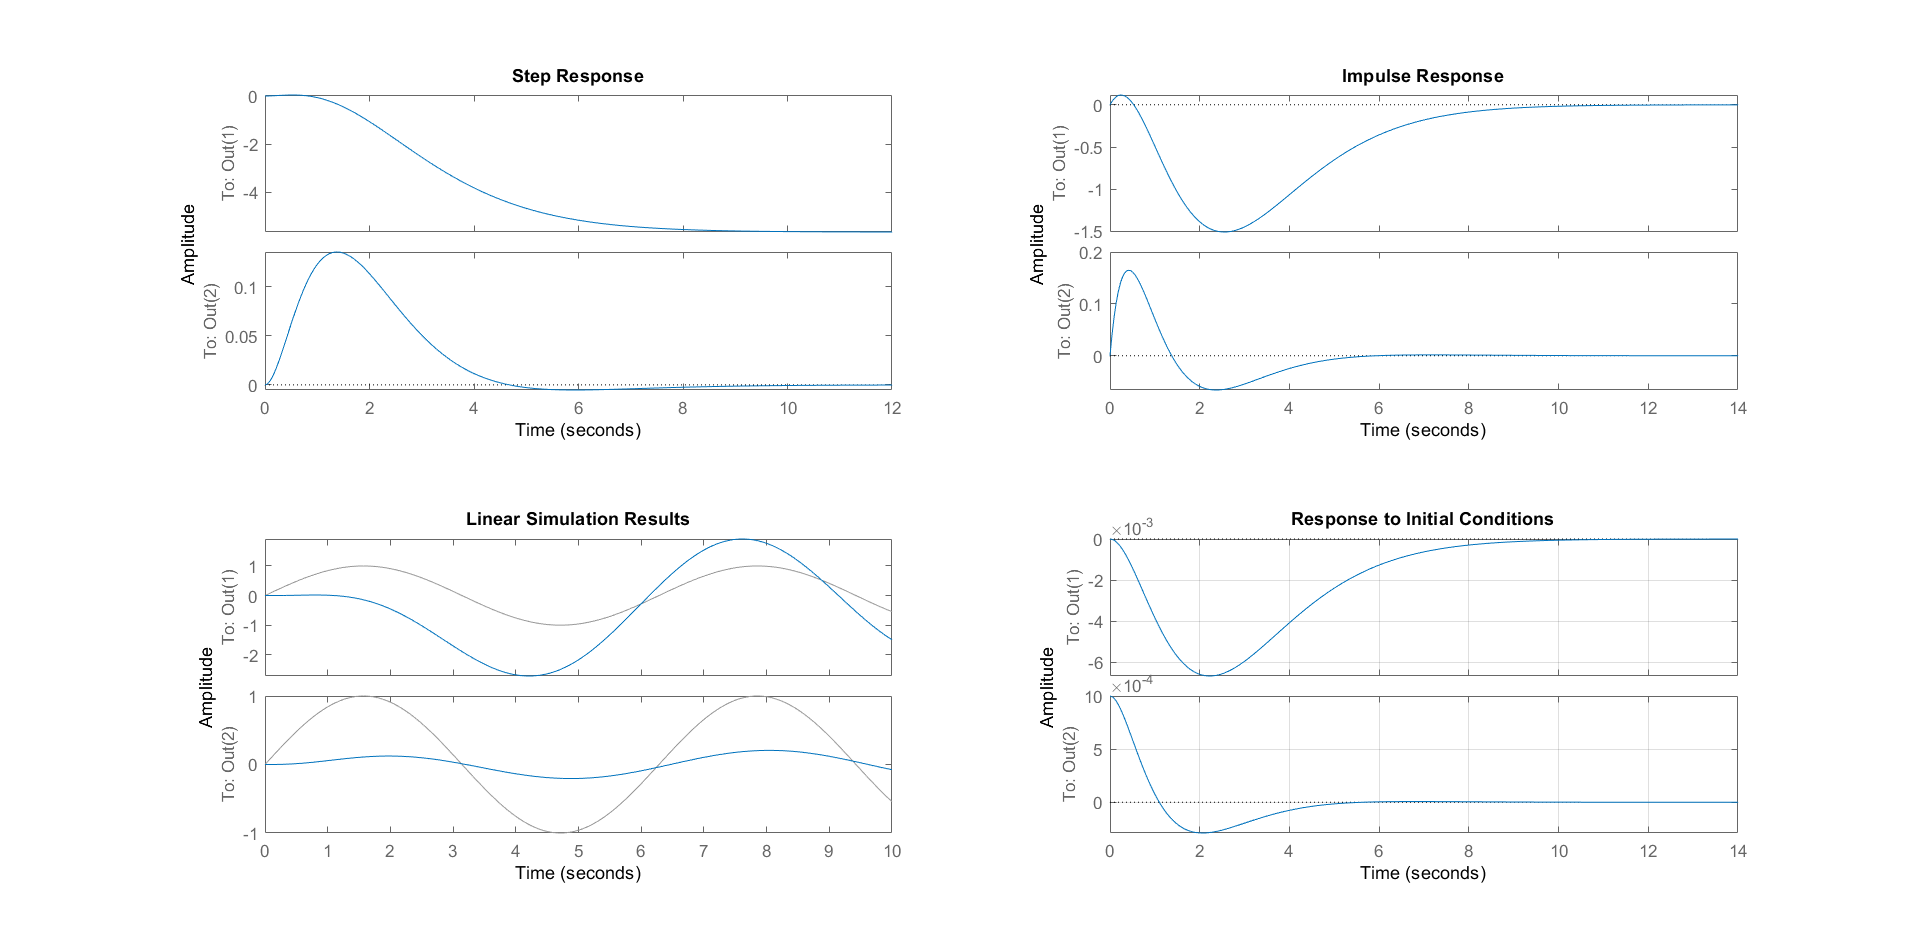
\includegraphics[width=10cm]{images/lin_cl_responses.png} \\
Αποκρίσεις γραμμικού κλειστού συστήματος
\end{center}


%----------------------------------------------------------------------------------------
%	ΓΡΑΜΜΙΚΟ ΜΟΝΤΕΛΟ ΜΕ ΘΟΡΥΒΟ ΚΑΙ ΦΙΛΤΡΟ KALMAN
%----------------------------------------------------------------------------------------

\section{Γραμμικό μοντέλο με θόρυβο και φίλτρο \textlatin{Kalman}}

Στην επόμενη μοντελοποίηση του συστήματος εισάγουμε θόρυβο στο πρότυπο του μοντέλου και στο πρότυπο των μετρήσεων. Υποθέτουμε οτι οι
οι θόρυβοι είναι προσθετικοί, λευκοί που ακολουθούν και ακολουθούν την κανονική κατανομή. Ο θόρυβος του συστήματος πρόερχεται από τριβές του εδάφους 
, του αέρα και του συνδέσμου, ενώ ο θόρυβος των μετρήσεων προέρχεται από σφάλματα των αισθητήρων.

\begin{center}
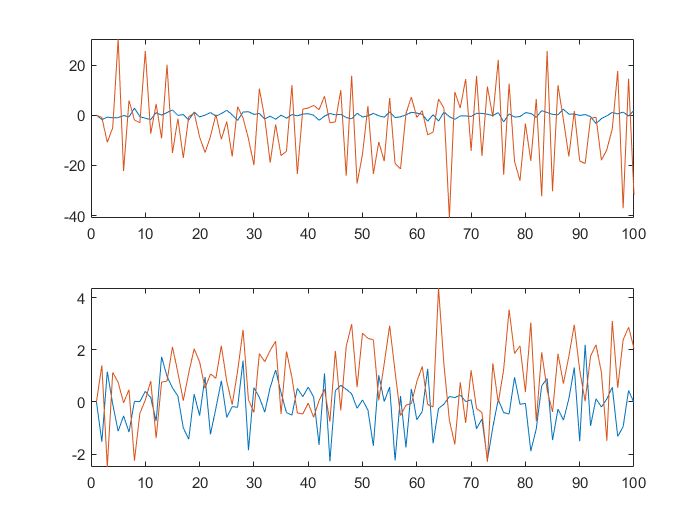
\includegraphics[width=10cm]{images/lin_model_measurements.png} \\
Μετρήσεις γραμμικού μοντέλου με θόρυβο
\end{center}

\[ w \sim N(0, Q) \;\; και \;\; υ \sim N(0,R) \]
όπου $$ R, Q $$ οι αντίστοιχοι πίνακες αυτοσυσχέτισης

\[
\begin{cases}
\dot{\vec{x}} = \mathbf{A}\vec{x} + \mathbf{B}u + \mathbf{G}w \\
\vec{y} = \mathbf{C}\vec{x} + \mathbf{D}u + υ
\end{cases}
\]

Εξισώσεις φίλτρου \textlatin{Kalman}:
\begin{enumerate}
	\item εξισώσεις πρόβλεψης
	\[ \hat{x}_{k|k-1} = \mathbf{A}_{k}\hat{x}_{k-1|k-1} + \mathbf{B}u_k \]
	\[ \mathbf{P}_{k|k-1} = \mathbf{A}_{k-1}\mathbf{P}_{k-1|k-1}\mathbf{A}_{k-1}^{\top} + \mathbf{G}_{k-1}\mathbf{R}_{w}(k-1)\mathbf{G}_{k-1}^{\top} \]
	\item εξισώσεις εκτίμησης και ανανέωση συμμεταβλητότητας σφάλματος
	\[ \mathbf{K}_k = \mathbf{P}_{k|k-1} \mathbf{H}_k^\top ( \mathbf{H}_k \mathbf{P}_{k|k-1} \mathbf{H}_k^\top + \mathbf{R}_υ(k) )^{-1} \]
	\[ \mathbf{P}_{k|k} = ( \mathbf{I} - \mathbf{K}_k\mathbf{H}_k ) \mathbf{P}_{k|k-1} \]
	\[ \hat{x}_{k|k} = \mathbf{A}_{k}\hat{x}_{k-1|k-1} + \mathbf{K}_k (y_k - \mathbf{H}_k \hat{x}_{k|k-1} ) \]
\end{enumerate}


%----------------------------------------------------------------------------------------
%	ΜΗ ΓΡΑΜΜΙΚΟ ΜΟΝΤΕΛΟ ΜΕ ΦΙΛΤΡΟ EKF
%----------------------------------------------------------------------------------------

\section{Μη-γραμμικό μοντέλο με φίλτρο \textlatin{EKF}}

Το μη γραμμικό σύστημα είναι της μορφής:
\[
\begin{cases}
\dot{\vec{x}} = f(\vec{x}, u) + \mathbf{G}w \\
\vec{y} = h(\vec{x}, u) + υ
\end{cases}
\]

το οποίο γραμμικοποιείται τοπικά ως εξής, προκειμένου να χρησιμοποιηθεί το \textlatin{EKF}
\[ 
\mathbf{F} = \frac{\partial f}{\partial \vec{x}} \biggr\rvert_{\hat{x}_{k-1}}^{} 
\mathbf{H} = \frac{\partial h}{\partial \vec{x}} \biggr\rvert_{\hat{x}_{k-1}}^{} 
\]
οπότε προκύπτει το εξής γραμμικοποιημένο σύστημα
\[
\begin{cases}
\delta \vec{x}_k = \mathbf{F}\delta\vec{x}_{k-1} + \mathbf{G}w_k \\
\delta \vec{y}_k = \mathbf{H}\delta\vec{x}_k + υ_k
\end{cases}
\]


Εξισώσεις φίλτρου \textlatin{EKF}
\begin{enumerate}
	\item εξισώσεις πρόβλεψης
	\[ \hat{x}_{k|k-1} = f(\hat{x}_{k-1|k-1}, u_k ) \]
	\[ \mathbf{P}_{k|k-1} = \mathbf{F}_{k-1}\mathbf{P}_{k-1|k-1}\mathbf{F}_{k-1}^{\top} + \mathbf{G}_{k-1}\mathbf{R}_{w}(k-1)\mathbf{G}_{k-1}^{\top} \]
	\item εξισώσεις εκτίμησης και ανανέωση συμμεταβλητότητας σφάλματος
	\[ \mathbf{K}_k = \mathbf{P}_{k|k-1} \mathbf{H}_k^\top ( \mathbf{H}_k \mathbf{P}_{k|k-1} \mathbf{H}_k^\top + \mathbf{R}_υ(k) )^{-1} \]
	\[ \mathbf{P}_{k|k} = ( \mathbf{I} - \mathbf{K}_k\mathbf{H}_k ) \mathbf{P}_{k|k-1} \]
	\[ \hat{x}_{k|k} = \mathbf{F}_{k}\hat{x}_{k-1|k-1} + \mathbf{K}_k (y_k - \mathbf{H}_k \hat{x}_{k|k-1} ) \]
\end{enumerate}


%----------------------------------------------------------------------------------------
%	ΜΗ ΓΡΑΜΜΙΚΟ ΜΟΝΤΕΛΟ ΜΕ ΦΙΛΤΡΟ UKF
%----------------------------------------------------------------------------------------

\section{Μη-γραμμικό μοντέλο με φίλτρο \textlatin{UKF}}

Εξισώσεις φίλτρου \textlatin{UKF}
\begin{enumerate}
	\item εξισώσεις πρόβλεψης
	\item εξισώσεις εκτίμησης και ανανέωση συμμεταβλητότητας σφάλματος
\end{enumerate}


%----------------------------------------------------------------------------------------
%	SENSOR FUSION
%----------------------------------------------------------------------------------------

%\section{\textlatin{Sensor Fusion}}






%----------------------------------------------------------------------------------------
%	ΒΙΒΛΙΟΓΡΑΦΙΑ, ΑΝΑΦΟΡΕΣ ΚΑΙ ΕΥΡΕΤΗΡΙΑ
%----------------------------------------------------------------------------------------

\nocite{*}
\printbibliography[heading=bibintoc,title={Βιβλιογραφία}]

%\end{otherlanguage}
\end{document}
